\chapter{Tau Multivariate Analysis}\label{sec:TauMVA}

The identification of taus that decay hadronically has been under extensive study to distinguish whether the custom tau multivariate analysis (tauMVA), the isolated track (isotrack) method, or the MVA from that is provided by the tau POG (tauPOG) has the highest efficiency to fake rate. The custom tauMVA was trained on PF charged hadron candidates with $\pt>10~\GeV$ and $|\eta|<2.4$ along with an additional PF photon candidate, if any, with $\pt>5$ GeV and within a cone of $\Delta R\leq0.2$ of the charged hadron candidate. The tau candidate is also required to have a transverse mass $m_T(\tau_h,\met)<100~\GeV$, where $m_T(\tau_h,\met)$ is defined as follows,
\begin{equation}\label{tauMT}
m_T(\tau_h,\met)=\sqrt{2\cdot\pt(\tau_h+\text{nearest}\gamma)\cdot\met\cdot(1-\cos\Delta\phi)}.
\end{equation}

The addition of photons in the final definition is due to the possibility of taus decaying to neutral pions. This improves the resolution for the hadronic tau candidate. The inputs for the MVA are as follows:
\begin{itemize}
	\item The \pt{} and $|\eta|$ of the $\tau$ candidate.
	\item The sum \pt{} of charged particles associated to the primary vertex within $\Delta R$ cones of sizes 0.1, 0.2, 0.3, and 0.4 around the $\tau$ candidate.
	\item The summed \pt{} of all particles within $\Delta R$ cones of sizes 0.1, 0.2, 0.3, and 0.4 around the candidate, now including the neutral contribution from pileup particles, which is reduced by applying the $\Delta \beta$ correction to the neutral component of the isolation quantity. 
	\item The distance in $\Delta R$ to the nearest charged PF candidate with $\pt>1~\GeV$.
	\item The distance in $\Delta R$ to the axis of the jet containing the $\tau$ candidate, and the b-tagging discriminant (DeepCSV) value for the jet, provided that the jet has $\pt>30~\GeV$ and $|\eta|<2.4$.
\end{itemize}

\begin{figure}
 	\centering
	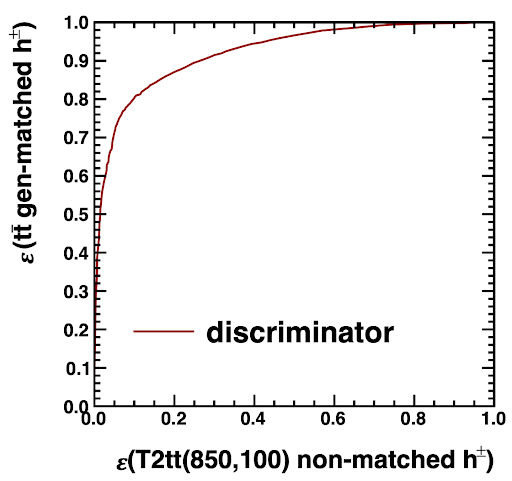
\includegraphics[width=0.60\textwidth]{tauMVA_ROCCurve.png}
 	\caption[Tau MVA ROC Curve]{A Receiver Operator Characteristic curve for the tauMVA discriminator.}
 	\label{tauMVAROCCurve} 
\end{figure}

\begin{figure}[!htb]
	\begin{center}
		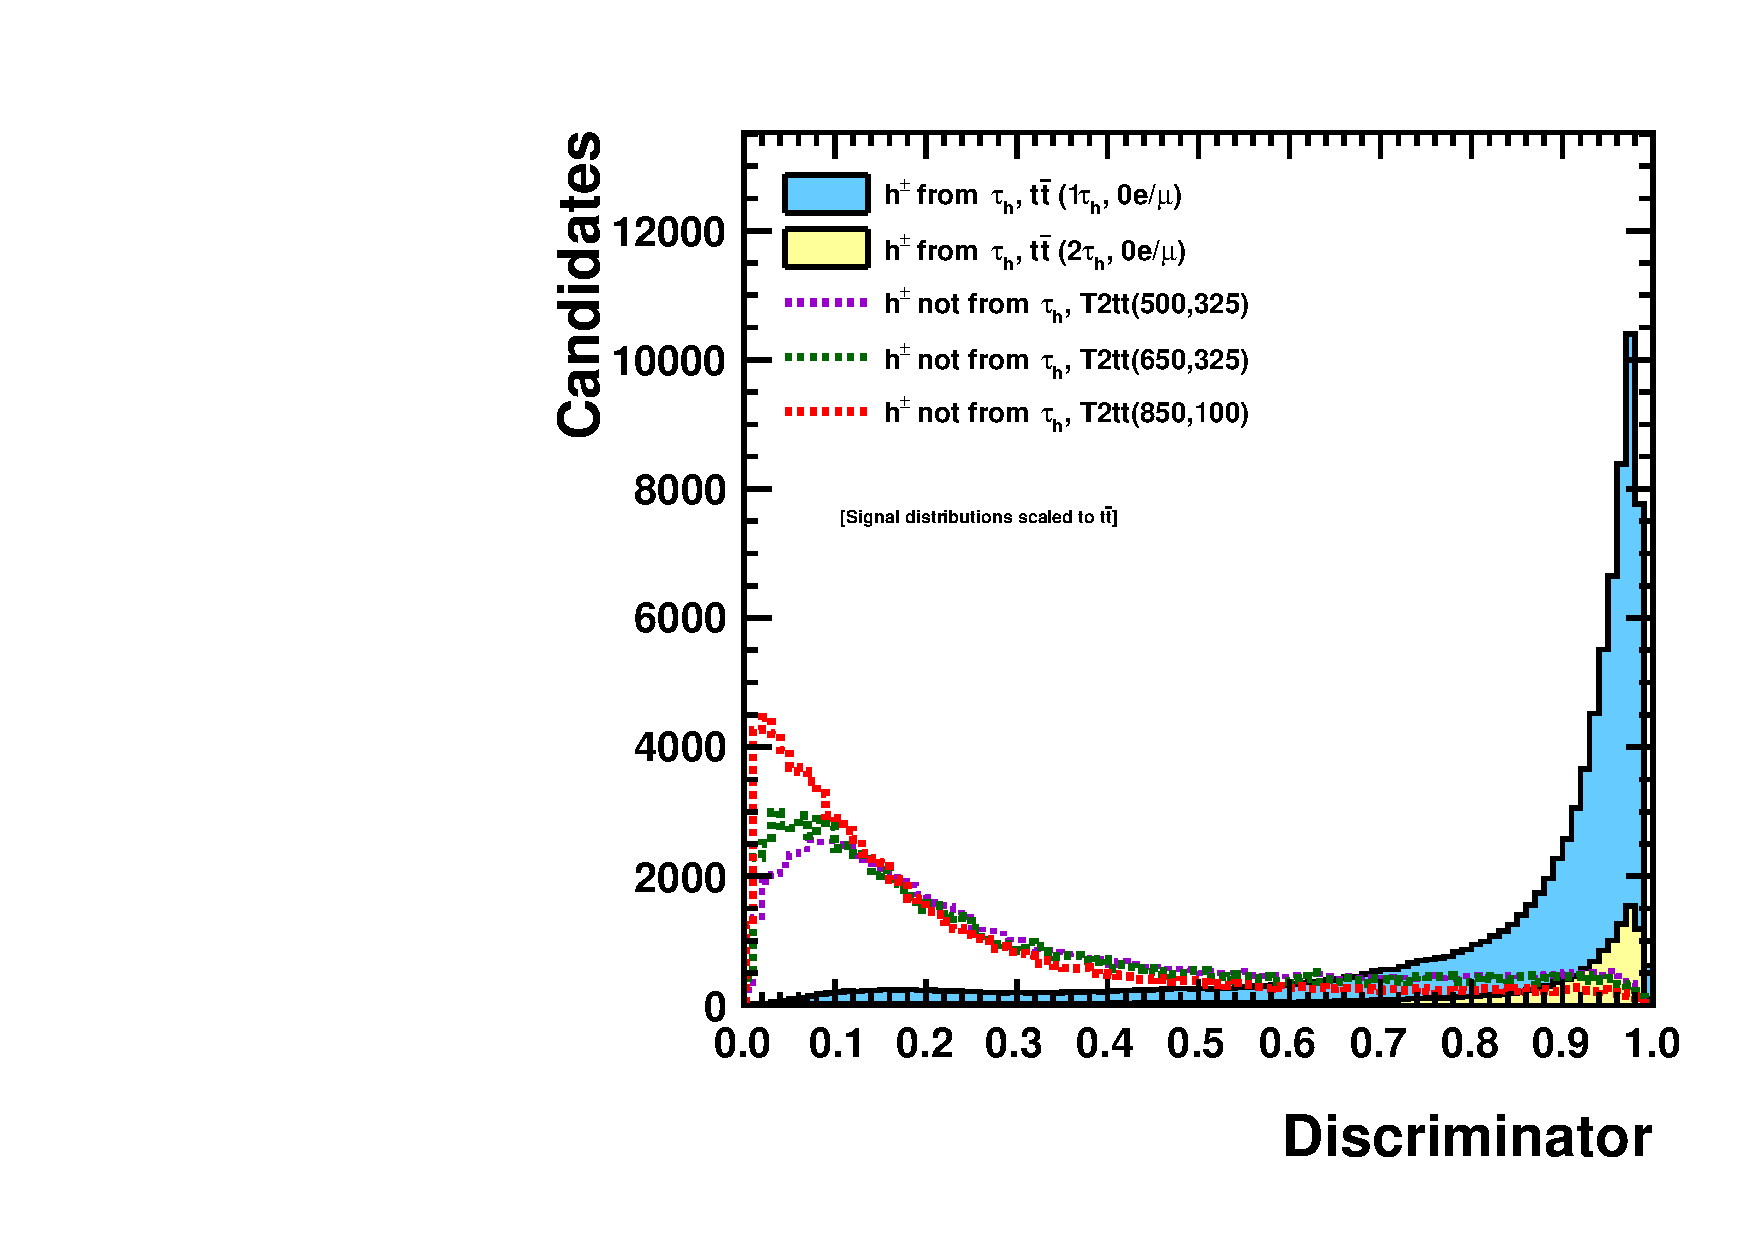
\includegraphics[width=0.5\textwidth]{mva_eta03_sigscalesumbkg_thesis.pdf}
		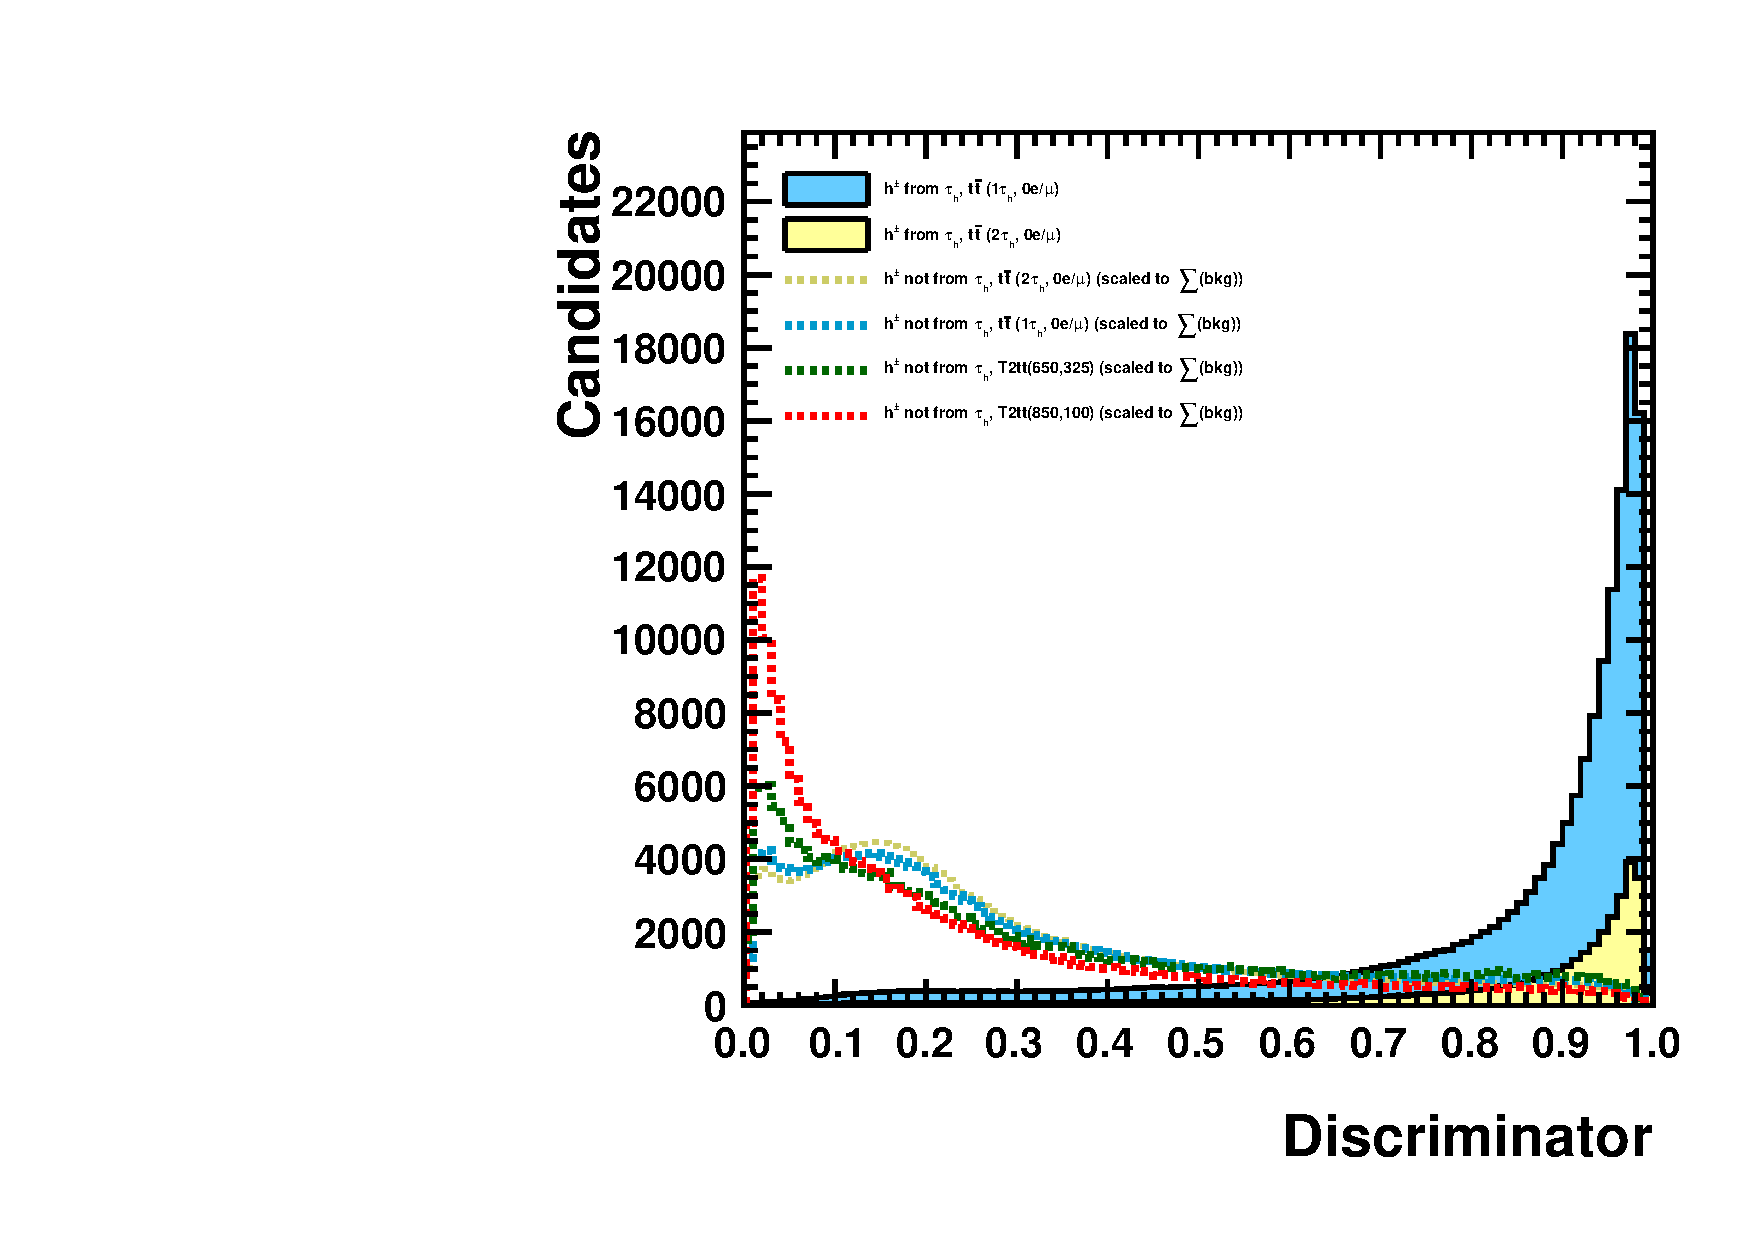
\includegraphics[width=0.5\textwidth]{mva_fakett_eta03_allpu_sigscalesumbkg_thesis.pdf} \\
	\end{center}
	\caption[Tau MVA Discriminator]{Tau MVA discriminator for different types of samples.
	}
	\label{fig:tau-discriminator}
\end{figure}

% matches pred table
% copy and paste the output from the end of LLBPred() (it calls printMoriond17Table) between the below labels "start insert" and "stop insert".
\begin{table}[!h]
\begin{center}
\resizebox*{\textwidth}{!}{
\begin{tabular}{|c||c||c|c|c||c|c|c|}
\hline
& & \multicolumn{3}{c||}{\ttbar{} 1-lepton} & \multicolumn{3}{c||}{\ttbar{} Di-lepton}\\
\hline
\hline
Type & Discriminator Cut & Efficiency & Fake Rate & Efficiency/Fake & Efficiency & Fake Rate & Efficiency/Fake \\
\hline
IsoTrack  & - & 27.9 \% & 6.1 \% & 4.541 & 24.8 \% & 6.1 \% & 4.084 \\
TauMVA & 0.68  & 34.9 \% & 6.9 \% & 5.046 & 24.7 \% & 5.3 \% & 4.689 \\
TauMVA & 0.70  & 34.6 \% & 6.5 \% & 5.355 & 24.4 \% & 4.9 \% & 4.997 \\
TauMVA & 0.71  & 34.4 \% & 6.2 \% & 5.525 & 24.2 \% & 4.7 \% & 5.170 \\
TauMVA & 0.73  & 33.9 \% & 5.7 \% & 5.914 & 23.8 \% & 4.3 \% & 5.540 \\
TauMVA & 0.74  & 33.6 \% & 5.5 \% & 6.119 & 23.6 \% & 4.1 \% & 5.712 \\
TauMVA & 0.75  & 33.4 \% & 5.2 \% & 6.356 & 23.4 \% & 3.9 \% & 5.961 \\
\hline 
\end{tabular}
}
\caption[TauMVA Background Optimization]{\label{tab:tau-mva-bkg}Comparing the efficiencies and Fake Rates of many difference discriminator cuts for the TauMVA and IsoTrack methods with SM simulation.}
\end{center}
\end{table}

\begin{table}[!h]
\begin{center}
\resizebox*{\textwidth}{!}{
\begin{tabular}{|c||c||c|c|c||c|c|c|}
\hline
& & \multicolumn{3}{c||}{T1tttt(2000,100)} & \multicolumn{3}{c||}{T2tt(850,100)}\\
\hline
\hline
Type & Discriminator Cut & Efficiency & Fake Rate & Efficiency/Fake & Efficiency & Fake Rate & Efficiency/Fake \\
\hline
IsoTrack  & - & 7.4 \% & 2.9 \% & 2.503 & 5.5 \% & 2.0 \% & 2.704 \\
TauMVA & 0.68  & 5.7 \% & 8.1 \% & 0.696 & 4.8 \% & 4.7 \% & 1.017 \\
TauMVA & 0.70  & 5.5 \% & 7.5 \% & 0.735 & 4.7 \% & 4.4 \% & 1.075 \\
TauMVA & 0.71  & 5.5 \% & 7.2 \% & 0.760 & 4.7 \% & 4.2 \% & 1.102 \\
TauMVA & 0.73  & 5.4 \% & 6.6 \% & 0.806 & 4.6 \% & 3.9 \% & 1.175 \\
TauMVA & 0.74  & 5.3 \% & 6.3 \% & 0.832 & 4.5 \% & 3.7 \% & 1.214 \\
TauMVA & 0.75  & 5.2 \% & 6.0 \% & 0.869 & 4.5 \% & 3.5 \% & 1.262 \\
\hline 
\end{tabular}
}
\caption[TauMVA Signal Optimization]{\label{tab:tau-mva-sig}Comparing the efficiencies and Fake Rates of many difference discriminator cuts for the TauMVA and IsoTrack methods with two SUSY simulations.}
\end{center}
\end{table}

\begin{table}[!h]
\begin{center}
\resizebox*{\textwidth}{!}{
\begin{tabular}{|c||c|c||c|c||c|c|}
\hline
& \multicolumn{2}{c||}{\ttbar{} 1-lepton} & \multicolumn{2}{c||}{T1tttt(2000,100)} & \multicolumn{2}{c|}{T2tt(850,100)} \\
\hline
\hline
Methods & Veto Percentage & Veto Efficiency & Veto Percentage & Veto Efficiency & Veto Percentage & Veto Efficiency \\
\hline
TauMVA         & 32.2\% & 57.7\% & 12.9 \% & 10.7 \% & 6.5\% & 10.9 \%  \\
IsoTrack        & 21.3 \% & 37.9 \% & 4.4 \% & 2.5 \% & 2.6 \% & 6.6 \%  \\
TauPOG         & 171 \% & 29.7 \% & 7.0 \% & 3.2 \%	& 5.2 \% & 2.5 \% \\
IsoTrack + TauPOG & 29.0 \% & 49.1 \% & 10.4 \% & 5.6 \% & 7.2 \% & 22.6 \% \\
\hline 

\end{tabular}
}
\caption[Tau Identification Comparisons]{\label{tab:tau-comparisons}Comparing the veto percentage and efficiency for the TauMVA, IsoTrack, TauPOG, and the IsoTrack + TauPOG methods with SM and SUSY simulations.}
\end{center}
\end{table}


In Figure \ref{tauMVAROCCurve}, we have a Receiver Operator Characteristic curve to compare the efficiency of the TauMVA in identifying taus that have been gen-level matched and the fake rate of tagging a parton as a tau that has not been gen-level matched. This shows that the TauMVA can potentially be a good discriminator of vetoing taus in our SM background while also not vetoing potential signal events. Then in Fig. \ref{fig:tau-discriminator}, we compare the TauMVA discriminator for events that have been matched to a gen-level tau (solid) and those that are not matched (dotted). We see good separation in events that are indeed a tau having a discriminator of approx. 1 and events that are not with a value of 0 to 0.2. This allows us to find a cut on the discriminator to maximize tagging real tau decays while also minimizing the fake taus.

Now that we have the definition for the TauMVA and have trained it on our samples to identify hadronically decaying taus. We want to compare the veto efficiencies and fake rates of the each method: TauMVA, IsoTrack, TauPOG, or a combination of IsoTrack and TauPOG. 
In Tables \ref{tab:tau-mva-bkg} and \ref{tab:tau-mva-sig}, we are comparing many different TauMVA cuts, $(>0.68, >0.70, >0.71, >0.73, >0.74, >0.75)$, with the IsoTrack method for \ttbar{} single lepton and dilepton SM samples, and T1tttt(2000, 100) and T2tt(850, 100) signal samples. The TauMVA cut of $MVA>0.71$ gives us the largest efficiency identifying gen taus, while also not vetoing fake taus from the signal events we are interested in analyzing.

In Table \ref{tab:tau-comparisons}, we are now comparing the TauMVA, IsoTrack, TauPOG, and IsoTrack + TauPOG methods for identifying hadronically decaying taus. The TauMVA and IsoTrack + TauPOG methods have very similar veto percentages and efficiencies for SM events, but the IsoTrack + TauPOG method has a similar or better veto percentage and efficiency for signal samples. Thus, our analysis has decided to use that as our tau ID, see Sec. \ref{TauID}.
